\chapter{Introducción}
\label{ch:1}

En este primer capítulo, se dará a conocer la motivación del proyecto, ofreciendo una perspectiva general del contexto y objetivos que lo atañen.

\section{Motivación}

En las últimas décadas, tanto el calentamiento global como el cambio climático se han visto  significativamente alentados por el crecimiento en la demanda energética de edificios residenciales y comerciales. De acuerdo con organizaciones como la Agencia Internacional de Energía\footnote{\url{https://www.iea.org/topics/buildings}} (\textit{International Energy Agency}, IEA), o WBCSD\footnote{\url{https://www.wbcsd.org/Programs/Cities-and-Mobility/Resources/Business-realities-and-opportunities-Summary}} (\textit{World Business Council for Sustainable Development}), los edificios y el sector de la construcción son responsables de más de un tercio del consumo mundial de energía, y de hasta un 40\% del total de las emisiones directas e indirectas de CO$_2$. 

Dichas emisiones, tras cierta estabilidad entre 2013 y 2016, alcanzaron su mayor nivel jamás registrado en 2019, produciéndose un crecimiento propiciado por múltiples factores, tales como la creciente demanda de energía destinada a sistemas de calefacción, ventilación y aire acondicionado (HVAC), el uso extendido de combustibles fósiles, la falta de políticas eficaces en eficiencia energética, así como una insuficiente inversión en edificios sostenibles\footnote{\url{https://www.iea.org/reports/tracking-buildings-2020}}.

Ante esta problemática, las propuestas más recientes destinadas a favorecer la eficiencia energética abogan, no sólo por fuentes de energía renovables, sino por la mejora en la gestión energética de las infraestructuras. Así quedó reflejado en el desafío \textit{Secure, Clean and Efficient Energy} del programa Horizonte2020 de la Unión Europea \cite{brenneche2012secure}, que planteaba entre sus objetivos la reducción del consumo energético y el desarrollo de áreas urbanas sostenibles dentro del marco de las \textit{Smart Cities}, así como en el clúster 5: \textit{Climate, Energy and Mobility} dentro del nuevo Horizonte Europa\footnote{\url{https://ec.europa.eu/info/research-and-innovation/funding/funding-opportunities/funding-programmes-and-open-calls/horizon-europe/cluster-5-climate-energy-and-mobility_en}}.

No obstante, la reducción en el consumo energético se ha visto obstaculizada por la demanda energética de los dispositivos HVAC en edificios residenciales y comerciales \cite{garcia2012heat}. Los sistemas HVAC se ocupan de regular la cantidad de energía destinada a la calefacción o refrigeración de los edificios para garantizar el \textit{comfort} de sus ocupantes. La optimización en el control de estos sistemas se plantea, pues, como un reto clave a abordar de cara garantizar la eficiencia energética de los edificios.

Para lograr este cometido, encontramos múltiples propuestas basadas en Ciencia de Datos \cite{molina2017data}. Se trata de una disciplina que ha demostrado tener un gran potencial en este ámbito, permitiendo extraer conocimiento implícito relacionado con la demanda energética de los dispositivos HVAC, así como con los factores externos que influyen en dicha demanda. En \cite{molina2017data} se muestra una panorámica de las principales aplicaciones de la Ciencia de Datos en control energético de edificios, las cuales incluyen:

\begin{itemize}
    \item Predicción de la demanda energética de los edificios.
    \item Optimización de su rendimiento energético.
    \item Análisis y reacondicionamiento de edificios.
    \item Prevención de fraudes.
    \item Análisis económico del consumo energético.
\end{itemize}

Con respecto a la optimización del rendimiento energético, en los últimos años el control HVAC ha sido abordado desde nuevas perspectivas más flexibles y eficientes que los sistemas de control clásicos. Este es el caso del Aprendizaje por Refuerzo (\textit{Reinforcement Learning}, RL) y su variante más actual: el Aprendizaje Profundo por Refuerzo (\textit{Deep Reinforcement Learning}, DRL), de especial utilidad y repercusión en control HVAC \cite{vazquez2019reinforcement}. Actualmente existen numerosas aplicaciones de DRL en este ámbito que han logrado mejorar los resultados ofrecidos por métodos de control convencionales, no sólo reduciendo el consumo energético de los edificios, sino garantizando al mismo tiempo el \textit{comfort} de sus ocupantes \cite{du2021intelligent,mckee2020deep,zhang2018practical}.

Sin embargo, a pesar de las múltiples ventajas que el DRL puede aportar en el control de dispositivos HVAC, se trata de un campo relativamente inmaduro, donde muy pocas propuestas en la literatura son realmente llevadas a la práctica, y donde se carece de  \textit{frameworks} específicamente destinados a reproducir y comparar los diferentes algoritmos que conforman el estado del arte. Tal y como Vázquez-Canteli \& Nagy \cite{vazquez2019reinforcement} evidencian en su reciente revisión de la literatura, la mayor parte de los trabajos en este ámbito son difícilmente reproducibles, lo que complica enormemente la comparación entre diferentes propuestas. Es necesario, por tanto, establecer un marco estandarizado que facilite la evaluación y comparativa de algoritmos de DRL en control HVAC. Este trabajo se presenta como una respuesta ante dicha necesidad.

\section{Objetivos}

Los \textbf{objetivos} que serán abordados en este trabajo son los siguientes:

\begin{tcolorbox}[colbacktitle=orange!30!white, title=Objetivo 1, coltitle=black, fonttitle=\bfseries]
Desarrollo de un entorno de ejecución de simulaciones energéticas adaptado para su uso con algoritmos de DRL.
\end{tcolorbox}

\begin{tcolorbox}[colbacktitle=orange!30!white, title=Objetivo 2,coltitle=black,fonttitle=\bfseries]
Integración, evaluación y comparativa de los resultados obtenidos por diferentes algoritmos de DRL sobre dicho entorno.
\end{tcolorbox}

Podemos desglosar dichos objetivos en los siguientes \textbf{subobjetivos}, los cuales se corresponderán con las actividades principales que se desarrollarán en el proyecto:

\begin{tcolorbox}[colbacktitle=orange!30!white, title=Subobjetivo 1, coltitle=black, fonttitle=\bfseries]
Comprensión de los fundamentos del aprendizaje por refuerzo y su aplicación en control HVAC.
\end{tcolorbox}

\begin{tcolorbox}[colbacktitle=orange!30!white, title=Subobjetivo 2, coltitle=black, fonttitle=\bfseries]
Extensión de la librería Python \href{https://github.com/jajimer/energym}{Energym} haciendo uso de la herramienta \href{https://gym.openai.com/}{Gym} de OpenAI.
\end{tcolorbox}

\begin{tcolorbox}[colbacktitle=orange!30!white, title=Subobjetivo 3, coltitle=black, fonttitle=\bfseries]
Entrenamiento monitorizado de diferentes algoritmos de DRL disponibles en \href{https://github.com/DLR-RM/stable-baselines3}{Stable Baselines3} haciendo uso de las herramientas \href{https://tensorflow.org/tensorboard}{TensorBoard} y \href{https://mlflow.org/}{MLflow}.
\end{tcolorbox}

\begin{tcolorbox}[colbacktitle=orange!30!white, title=Subobjetivo 4, coltitle=black, fonttitle=\bfseries]
Comparativa de los resultados obtenidos para cada uno de los agentes en diferentes contextos de clima y espacios de acciones (discreto y continuo).
\end{tcolorbox}

\begin{tcolorbox}[colbacktitle=orange!30!white, title=Subobjetivo 5, coltitle=black, fonttitle=\bfseries]
Estudio de la recompensa obtenida por un agente en función de la importancia asignada a confort y consumo energético.
\end{tcolorbox}

\begin{tcolorbox}[colbacktitle=orange!30!white, title=Subobjetivo 5, coltitle=black, fonttitle=\bfseries]
Ejecución de pruebas de robustez que permitan conocer el rendimiento de los agentes en diferentes climas a los empleados como entrenamiento.
\end{tcolorbox}

\begin{tcolorbox}[colbacktitle=orange!30!white, title=Subobjetivo 5, coltitle=black, fonttitle=\bfseries]
Aplicación de \textit{curriculum learning} con diferentes agentes y análisis de los resultados obtenidos.
\end{tcolorbox}

\section{Planificación}

Para llevar a cabo el desarrollo de este proyecto se optó por seguir una metodología \textbf{Agile Data Science} \cite{jurney2017agile}, basada en una serie de principios clave como el desarrollo iterativo, la continua comunicación con el equipo de trabajo y entrega de prototipos intermedios que permitan al cliente (en este caso, los tutores del proyecto) conocer el estado de su desarrollo. Como se detallará en el Capítulo \ref{ch:3}, la realización de este proyecto supuso la integración en un equipo de trabajo profesional y la adaptación a un método de desarrollo basado en la aportación al proyecto mediante \textit{pull requests} e \textit{issues} de GitHub, \textit{integración continua} (CI) y otras prácticas habituales en el marco \textit{DevOps}.

Con respecto a la \textbf{planificación temporal} del proyecto, en la Figura \ref{fig:planning} se muestra el reparto de días de trabajo y la distribución de las diferentes tareas abordadas. Estas se corresponden con la consecución de los objetivos y subobjetivos anteriormente planteados. Tal y como se muestra en la figura, la duración del proyecto ha sido de un total de \textbf{160 días}. Se estima un total de \textbf{320 horas} de trabajo, lo cual se ajusta a las 300 horas correspondientes a un Trabajo de Fin de Máster de 12 créditos.

\begin{figure}
    \centering
    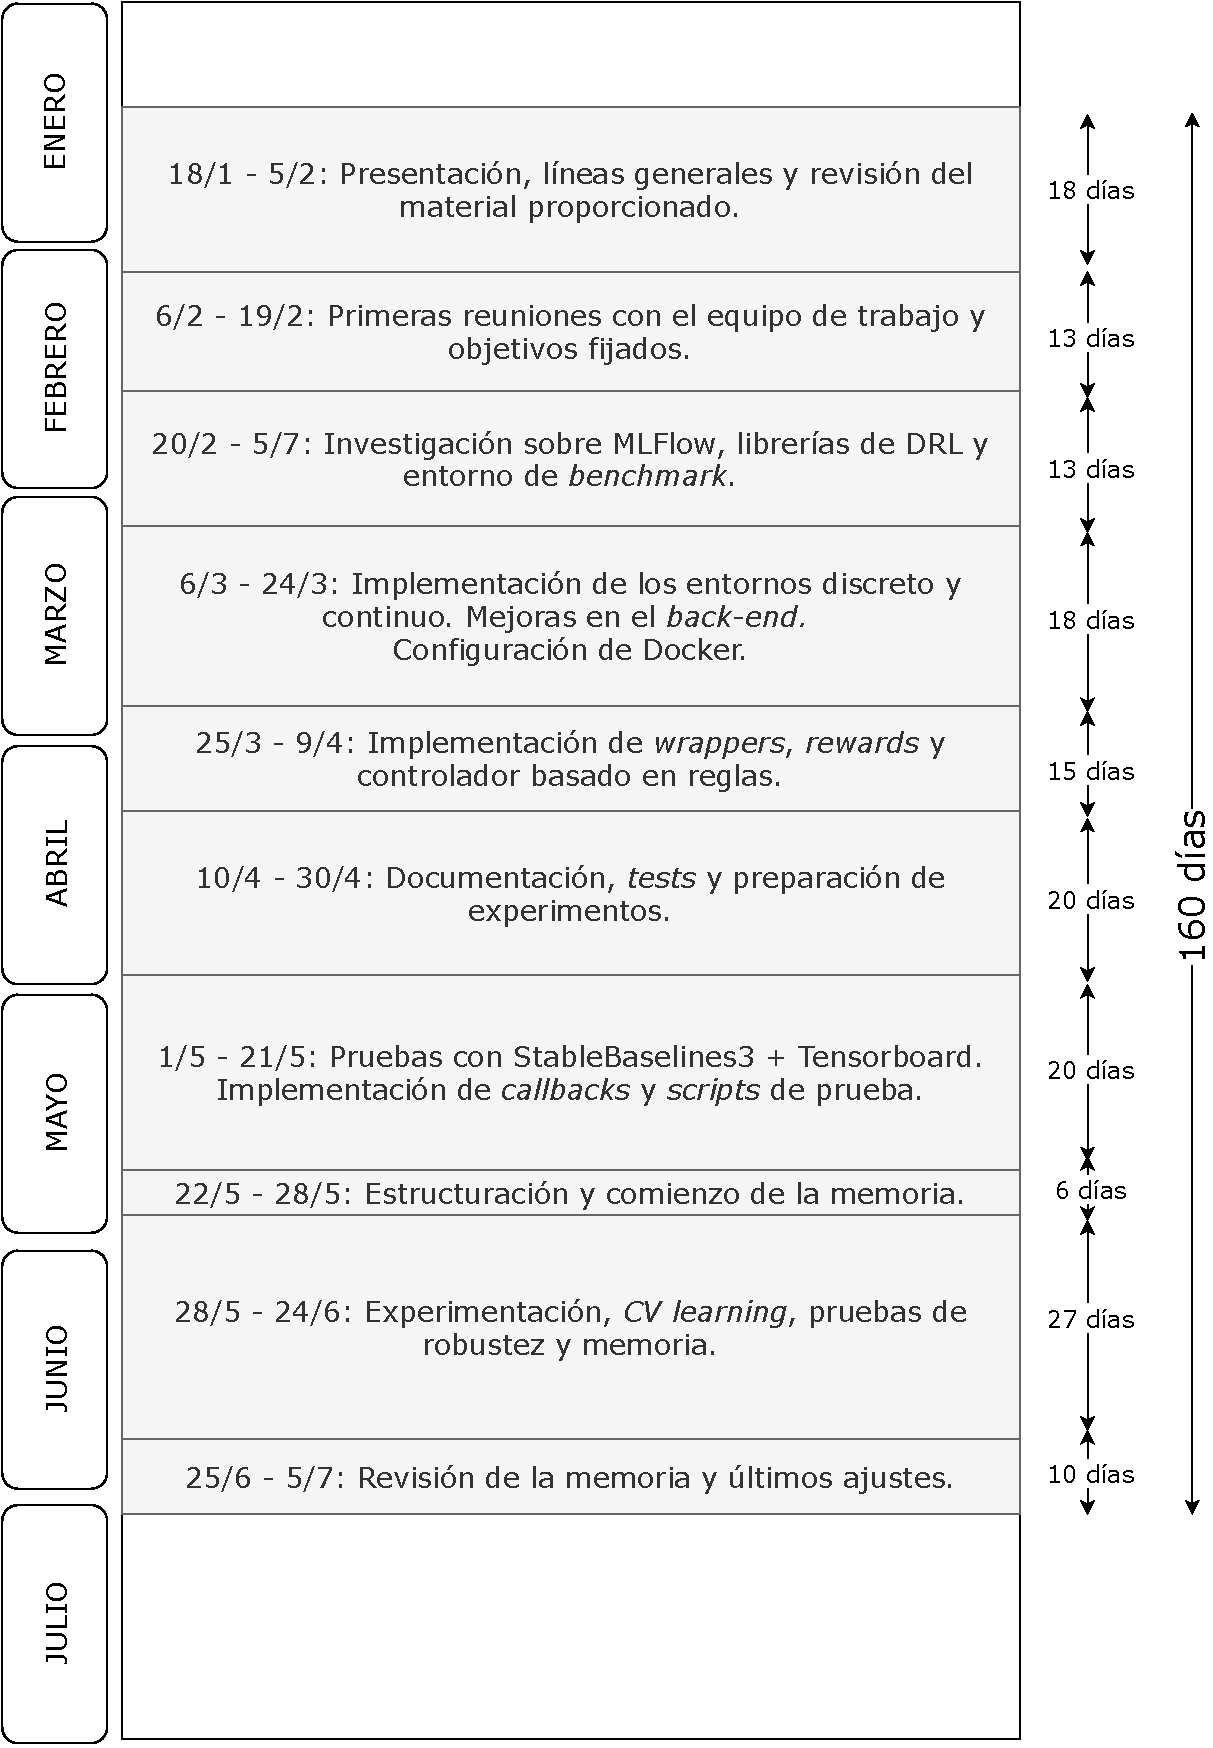
\includegraphics[width=\textwidth]{imagenes/planning.pdf}
    \caption{Planificación del proyecto}
    \label{fig:planning}
\end{figure}

Desde el punto de vista económico, los \textbf{gastos del proyecto} son los que se muestran en la Tabla \ref{tb:economico}. Algunos aspectos a considerar en su cálculo:

\begin{itemize}
    \item La estimación del coste por horas de trabajo se ha hecho de acuerdo a un salario medio aproximado de científico de datos de $25.000$ \euro\ según la plataforma \href{https://www.glassdoor.es/}{Glassdoor} a fecha de Junio de 2021.
    \item Los porcentajes de cotización a la seguridad social fueron obtenidos desde la web del \href{https://www.seg-social.es/wps/portal/wss/internet/Trabajadores/CotizacionRecaudacionTrabajadores/36537}{Ministerio de Inclusión, Seguridad Social y Migraciones} a fecha de Junio de 2021.
    \item El IRPF ha sido calculado mediante la herramienta online proporcionada por \href{https://cincodias.elpais.com/herramientas/calculadora-irpf/}{CincoDías} para un ingeniero de 23 años, con sueldo bruto anual de $25.000$ \euro.
    \item Por otro lado, en la estimación de costes indirectos se han tenido en cuenta el consumo eléctrico medio y el \textit{hardware} empleado.
\end{itemize}

Así, con una duración aproximada de 6 meses, el \textbf{coste total} del proyecto se estima en 2.574,00 $\times$ 6 $=$ 15.444,00 \euro.

\begin{table}
    \centering
    \caption{Desglose de gastos del proyecto}
    \label{tb:economico}
    \resizebox{\textwidth}{!}{%
    \begin{tabular}{|l|c|}
    \hline
    \textbf{Variable} & \textbf{Valor} \\ \hline
    Sueldo bruto anual (\euro) & 25.000 \\ \hline
    Número de pagas (\euro) & 6 \\ \hline
    Sueldo bruto mensual (\euro) & 2.083,33 \\ \hline
    Cotización a la seguridad social (\% empresa) & 23,60 \\ \hline
    Cotización a la seguridad social (\% trabajador) & 4,70 \\ \hline
    IRPF (\%) & 14,28 \\ \hline
    \textbf{Sueldo neto mensual del empleado} (\euro) & \textbf{1.687,91} \\ \hline
    \textbf{Coste mensual para la empresa} (\euro) & \textbf{2.574,00} \\ \hline
    \end{tabular}%
    }
\end{table}

\section{Estructura}

Una vez definidos los objetivos del proyecto, en el Capítulo \ref{ch:2} abordaremos los fundamentos del aprendizaje por refuerzo y sus aplicaciones en control HVAC según el estado del arte. Posteriormente, en el Capítulo \ref{ch:3} se definirá el entorno de simulación \textit{Energym}, así como las aportaciones realizadas al mismo a lo largo de este proyecto. En el Capítulo \ref{ch:4} se describirán los principales resultados obtenidos tras la experimentación con diferentes agentes y entornos. Finalmente, en el Capítulo \ref{ch:5} abordaremos las conclusiones, trabajo futuro y lecciones aprendidas tras el desarrollo de este proyecto.

Todo el código empleado y al que haremos referencia a lo largo de este documento puede encontrarse en el siguiente repositorio de GitHub: \url{https://github.com/manjavacas/drl-building}. También puede consultarse la documentación de la librería \textit{Energym} elaborada durante el desarrollo de este trabajo: \url{https://energym.readthedocs.io/}, así como su código fuente: \url{https://github.com/jajimer/energym}.

